\chapter{AMR and LES}\label{amrles}
As mentioned in the last chapter, in LES we try to solve the FE
instead of the UE and treat the unresolved scales with a subgrid scale model,
which acts like a filter with a characteristic length $l_{\Delta}$ for the UE.
However we can only model the subgrid scales in an averaging sense, which can
only be correct, if the fluid motions on the subgrid scales are nearly
isotropic. This limits the LES methodology to flows where we can resolve all
anisotropies, which stem from large-scale features like boundary conditions or
external forces. Therefore the ideal numerical method for LES would include
adaptive gridding to ensure automatically that the grid, and hence the filter,
are everywhere sufficiently fine to resolve the energy-containing motions
\citep[p. 636]{Pope2000}.

\section{Adaptive mesh refinement}\label{amr}
The most powerful technique for grid-based solvers to resolve localized
and anisotropic structures in a flow is adaptive mesh refinement (AMR). 
Using AMR the grid will be refined\footnote{Refined means that the values from a
coarse parent grid are interpolated onto a finer child grid and then
integrated independently from the coarse grid. However, the way how to
interpolate the values from coarse to fine grid is not discussed in the
literature and most often not described by the developers of AMR fluid codes.
Although outside the scope of our work, the dependence of the solution and the
spectrum of the solution on this interpolation routines should be investigated
in the future.}, depending on a refinement criterion, only at
the defined ``interesting'' areas of the flow field. This allows for
treating a much bigger range of dynamic scales of the fluid with the same
number of grid cells compared to a static grid.

\begin{figure}[tp]
\centering
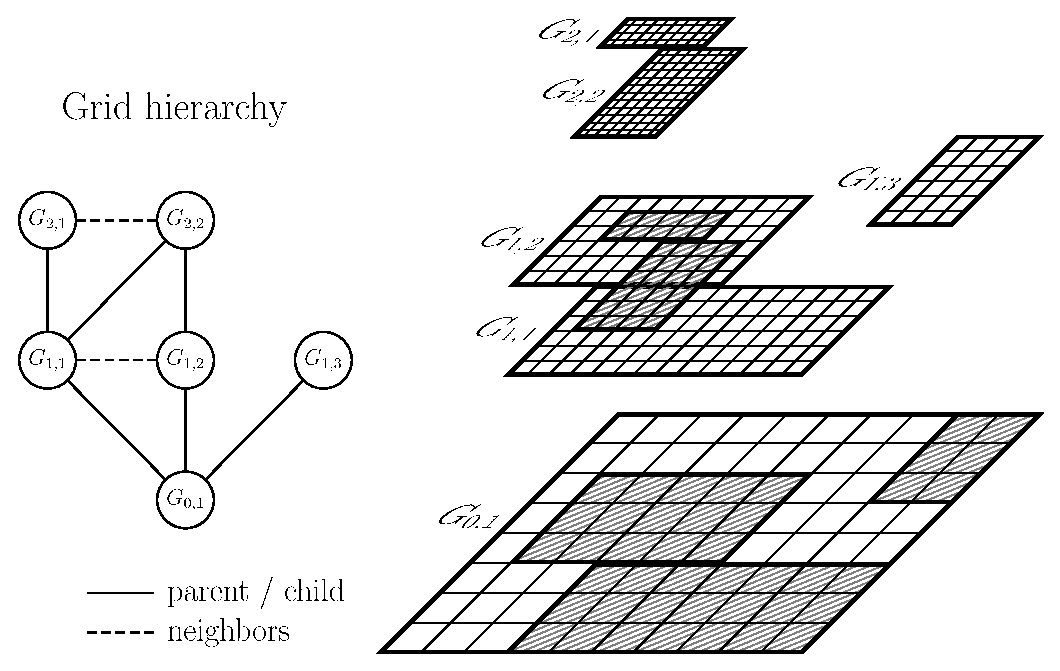
\includegraphics[width=0.7\linewidth]{chapter6/blockamr.eps}
\caption{Hierarchy of rectangular subgrids in blockstructured
AMR \citep{Deiterding2003}.}
\label{fig:amr}
\end{figure}

The grid structure can thereby
be understood as a hierarchy of grid patches (see figure \ref{fig:amr}) that
approximate the flow on various levels of resolution
\citep{Berger1984,Berger1989}. But not only the spatial resolution, also
the time resolution is adaptive. All grids on
a given level are advanced simultaneously with a
maximum timestep such that the Courant condition is
satisfied by all the cells on that level. This results in
a hierarchy of timesteps: a coarse, parent grid on level $l$ is advanced by
$\Delta t^{\text{coarse}}$, and then its finer, subgrid(s) on level $l + 1$ are
advanced by one or more timesteps $\Delta t^{\text{fine}}$ until they reach
the same physical time as their parent grid. 
At this point, the coarse grid values $u^{\text{coarse}}$ are replaced by the
underlying fine grid values $u_i^{\text{fine}}$ using mass weighted,
conservative averaging\footnote{Density itself is not weighted by mass but only
by volume $\rho^{\text{coarse}}=\frac{1}{V}\sum_i \rho_i^{\text{fine}} V_i$.} 
\begin{align}
u^{\text{coarse}}=\frac{1}{M}\sum_i \rho_i u_i^{\text{fine}} V_i,
\end{align}
where $M=\sum_i \rho_i V_i$ is the total mass of the underlying subgrid cells
and $V_i$ is the volume of a fine grid cell. 

To completely ensure mass conservation, however, one not only has to replace the
coarse grid values with averaged fine grid values, but also must correct
coarse grid cells, which abut fine grid cells, but are not themselves
covered by any fine grid. This can be understood, by writing the underlying, 
conservative, explicit finite difference scheme as
\begin{align}
u_n(t+\Delta t^{\text{coarse}}) = u(t) 
- \frac{\Delta t^{\text{coarse}}}{\delta x}
\lra{F^{\text{coarse}}_{n+1/2}-F^{\text{coarse}}_{n-1/2}},\label{eq:finitediff}
\end{align}
where $F_{n \pm 1/2}$ are the fluxes on the left and right hand
side of the cell number $n$ respectively. If the left hand side of cell $n$
abuts on a fine grid, the flux $F^{\text{coarse}}_{n-1/2}$ has to be replaced
by the fluxes of the neighboring fine grid cells
\begin{align}
F^{\text{fine}}_{n-1/2}=\sum_i F_{i+1/2}(t+i \Delta t^{\text{fine}}),
\end{align}
where the sum is due to the refinement in time. This flux replacement is most
often implemented as a correction pass after a grid has been integrated using 
equation \ref{eq:finitediff}
\begin{align}
u_n(t+\Delta t^{\text{coarse,corr}}) = 
u_n(t+\Delta t^{\text{coarse}}) + \Delta F
\end{align}
with 
\begin{align}
\Delta F = -F^{\text{coarse}}_{n-1/2}+
\sum_i F_{i+1/2}(t+i \Delta t^{\text{fine}}).
\end{align}
This "Flux Correction" step is the most difficult and error-prone part of an
AMR implementation, since one has to track all the fluxes of the time varying
boundaries of coarse and fine grids, and correctly maintain them between
processors, if the simulation is run in parallel on several CPUs.   

Nevertheless, if done correctly, this technique has proven to be very well
suited for astrophysical problems which include strong
shocks or gravitational collapse \citep{Bryan2001} among many other
applications. However, in the case of astrophysically relevant Reynolds
numbers\footnote{See section \ref{kolmo}.} even with AMR we cannot hope to
resolve all relevant scales down to the dissipative scales
\citep{Schmidt2006a}.

But as mentioned in the introduction, we do not have to
resolve all scales if we use a SGS model. We only need to resolve
energy-containing motions. That's the reason why combining LES and AMR offers
the
possibility of treating turbulence in astrophysical simulations in a much better
way. Though there is one big problem, when trying to combine LES with AMR. Most
of the terms of a SGS model like the Schmidt model do depend on the
cutoff scale $l_{\Delta}$ of the grid and this cutoff scale varies in time and
space if one uses AMR. But when filtering the fluid dynamic equations, we
assumed our filter operation to commute with time and spatial derivatives and
hence be static and isotropic, in direct contradiction to the methods of AMR.
Therefore combining LES and AMR seem to pose a big challenge and only few
attempts have been made so far.

\section{Attempts to combine LES and AMR}
Although proposals to combine LES and AMR are frequently made
(e.g \citet{Pope2004}), literature on the topic is still rare.

Probably the first attempt to combine LES and AMR is due to
\citet{Sullivan1996}. They used a kind of zero-filling to interpolate
the solution between the coarse and fine grid. But their simulation of
planetary boundary layers only used one static nested fine grid within a coarse
grid and was therefore of limited use for more general problems.
\citet{Boersma1997} came to the conclusion, using the methods of
\citet{Sullivan1996}, that with respect to statistics, the nested grid
simulations are clearly superior to the results obtained with a simulation on a
coarse grid in the whole flow domain. They also found that their
solution of a 2d Kelvin-Helmholtz instability improves even in the area only
covered by the coarse grid, an encouraging fact. Another approach to large eddy
simulations using AMR was put forward by \citet{Cook1999}. He presented a
method for computing a fine grid solution given a coarse grid solution and vice
versa using a deconvolution with a gaussian filter. He showed how to avoid
commutation errors with this technique, and that boundary errors are usually
small. He also emphasized the advantage of using several nested grids instead
of one stretched grid. He came to the conclusion, however, that shocks and
other 
high-frequency phenomena should not be allowed to cross grid boundaries, which
renders his method invalid for simulating compressible flows in astrophysics. 

A sophisticated approach is the multilevel algorithm for large-eddy
simulation of turbulent flow by \citet{Terracol2001,Terracol2003}.
\footnote{Also see the book of \citet{Sagaut2006a}.} But although
they use a time-dependent number of grids, the finer grids in their simulations
always cover the whole computational domain and and are only used to improve
the overall LES performance. Also methods based on wavelets have been proposed
by \citet{Goldstein2004} and \citet{Leonard2006} and even for
adaptive, unstructured grids \citep{Mitran2001a, Naegele2003}, but
seem to be
rarely used. The newest method to combine LES and blockstructured AMR comes from
\citet{Pantano2007}, but they use a very different SGS-model compared to the
Schmidt model considered in our work and therefore it is unclear if their
method is of general use.

Finally in an astrophysical context \citet{Falle1994} claims to use a
$k$-$\epsilon$ subgrid scale model build into the hierarchical adaptive grid
code $\mu$Cobra to treat the effect of turbulence on the large structure of
radio jets. However the specific problems due to adaptive gridding are not
mentioned in this paper and \citet{Falle1994} himself comes to the conclusion
that his treatment of turbulence is rather dubious. Nevertheless, the same model
seems to be used in a recent paper by \citet{Pope2008} on the generation of
optical emission-line filaments in galaxy clusters. 

\section{\texorpdfstring{$\epsilon$}{epsilon}-based approach to combine AMR and
LES}\label{epsilon}
In this chapter, we want to present a new simple method to address the problem
of combination of AMR and LES. It is based on the finding of section
\ref{ImpactSGS}, that the turbulent dissipation $\epsilon$ is related to the
dissipation scale, but in the Schmidt model (and most other SGS models) modeled
depending on the cutoff scale. This is no problem, if we use a static grid in
our fluid dynamic simulation, but it poses a problem in AMR simulations. The
reason is that the time and spatial variance of $l_{\Delta}$ in an adaptive
simulation leads to an artificial dependence of $\epsilon$ on the grid
structure of the simulation. But as we now from Kolmogorovs theory of turbulence
the average rate of dissipation should be independent of the length scale in
fully developed turbulence. This would not be the case in a AMR simulation of
fully developed turbulence, if $\epsilon$ depends on the cutoff scale, since
the average turbulent energy and therefore the turbulent velocity $q$ is 
independent of the lengthscale in a conservative AMR code. So our idea is to
try to enforce the independence of $\epsilon$ on the grid patches of different
cutoff scale in our AMR simulations of turbulence. Explicitely this can be
written as
\begin{align}
\epsilon(l_{\Delta,1})=\epsilon(l_{\Delta,2}),\
l_{\Delta,1} > l_{\Delta,2}
\end{align}
where $\epsilon(l_{\Delta,1})$ is the value of the turbulent dissipation in
one grid cell of the coarse grid and $\epsilon(l_{\Delta,2})$ is the average 
value of the turbulent dissipation after interpolation on a overlapping fine
grid patch.  
Inserting our model for epsilon \eqref{eq:epsmodel} we get
\begin{align}
C_{\epsilon,1}\frac{q_1^3}{l_{\Delta,1}}=
C_{\epsilon,2}\frac{q_2^3}{l_{\Delta,2}}.
\end{align}
Assuming $C_{\epsilon,1}=C_{\epsilon,2}$ this leads to
\begin{align}
\frac{q_1^2}{q_2^2}=\lra{\frac{l_{\Delta,1}}{l_{\Delta,2}}}^{2/3},
\label{eq:qscale}
\end{align}
which is a scaling relation for the turbulent energy. This scaling relation
should hold between the turbulent energy on grid patches of different cutoff
scale. But on the other side, the total energy must be locally conserved
\begin{align}
\frac{1}{2}v_1^2 + \frac{1}{2}q_1^2 + u_1 = 
\frac{1}{2}v_2^2 + \frac{1}{2}q_2^2 + u_2.
\end{align}
Since in a conservative AMR code $u_1 = u_2$ and using the scaling relation
\eqref{eq:qscale} to eliminate $q_2$ we get
\begin{align}
v_2^2=v_1^2+q_1^2 \lra{1-r^{-2/3}},\label{eq:boostekin}
\end{align}
where we introduced the refinement factor
$r=\frac{l_{\Delta,1}}{l_{\Delta,2}}$. 
If we divide \eqref{eq:boostekin} by $v_1^2$ and assume isotropy, we can derive
a relation for the components of velocity 
\begin{align}
v_{2,i}=v_{1,i} \sqrt{1+\frac{q_1^2}{v_1^2} \lra{1-r^{-2/3}}}.
\end{align}
If we write equation \eqref{eq:qscale} like
\begin{align}
q_2^2 = q_1^2 - q_1^2 \lra{1-r^{-2/3}}
\end{align}
we see, that for infinite refinement $r \rightarrow \infty$ the turbulent
velocity  $q_2$ is zero as expected. 

